
%% bare_conf.tex
%% V1.4b
%% 2015/08/26
%% by Michael Shell
%% See:
%% http://www.michaelshell.org/
%% for current contact information.
%%
%% This is a skeleton file demonstrating the use of IEEEtran.cls
%% (requires IEEEtran.cls version 1.8b or later) with an IEEE
%% conference paper.
%%
%% Support sites:
%% http://www.michaelshell.org/tex/ieeetran/
%% http://www.ctan.org/pkg/ieeetran
%% and
%% http://www.ieee.org/

%%*************************************************************************
%% Legal Notice:
%% This code is offered as-is without any warranty either expressed or
%% implied; without even the implied warranty of MERCHANTABILITY or
%% FITNESS FOR A PARTICULAR PURPOSE! 
%% User assumes all risk.
%% In no event shall the IEEE or any contributor to this code be liable for
%% any damages or losses, including, but not limited to, incidental,
%% consequential, or any other damages, resulting from the use or misuse
%% of any information contained here.
%%
%% All comments are the opinions of their respective authors and are not
%% necessarily endorsed by the IEEE.
%%
%% This work is distributed under the LaTeX Project Public License (LPPL)
%% ( http://www.latex-project.org/ ) version 1.3, and may be freely used,
%% distributed and modified. A copy of the LPPL, version 1.3, is included
%% in the base LaTeX documentation of all distributions of LaTeX released
%% 2003/12/01 or later.
%% Retain all contribution notices and credits.
%% ** Modified files should be clearly indicated as such, including  **
%% ** renaming them and changing author support contact information. **
%%*************************************************************************


% *** Authors should verify (and, if needed, correct) their LaTeX system  ***
% *** with the testflow diagnostic prior to trusting their LaTeX platform ***
% *** with production work. The IEEE's font choices and paper sizes can   ***
% *** trigger bugs that do not appear when using other class files.       ***                          ***
% The testflow support page is at:
% http://www.michaelshell.org/tex/testflow/



\documentclass[conference]{IEEEtran}
% Some Computer Society conferences also require the compsoc mode option,
% but others use the standard conference format.
%
% If IEEEtran.cls has not been installed into the LaTeX system files,
% manually specify the path to it like:
% \documentclass[conference]{../sty/IEEEtran}


% Some very useful LaTeX packages include:
% (uncomment the ones you want to load)


% *** MISC UTILITY PACKAGES ***
%
%\usepackage{ifpdf}
% Heiko Oberdiek's ifpdf.sty is very useful if you need conditional
% compilation based on whether the output is pdf or dvi.
% usage:
% \ifpdf
%   % pdf code
% \else
%   % dvi code
% \fi
% The latest version of ifpdf.sty can be obtained from:
% http://www.ctan.org/pkg/ifpdf
% Also, note that IEEEtran.cls V1.7 and later provides a builtin
% \ifCLASSINFOpdf conditional that works the same way.
% When switching from latex to pdflatex and vice-versa, the compiler may
% have to be run twice to clear warning/error messages.






% *** CITATION PACKAGES ***
%
%\usepackage{cite}
% cite.sty was written by Donald Arseneau
% V1.6 and later of IEEEtran pre-defines the format of the cite.sty package
% \cite{} output to follow that of the IEEE. Loading the cite package will
% result in citation numbers being automatically sorted and properly
% "compressed/ranged". e.g., [1], [9], [2], [7], [5], [6] without using
% cite.sty will become [1], [2], [5]--[7], [9] using cite.sty. cite.sty's
% \citep{•}\cite will automatically add leading space, if needed. Use cite.sty's
% noadjust option (cite.sty V3.8 and later) if you want to turn this off
% such as if a citation ever needs to be enclosed in parenthesis.
% cite.sty is already installed on most LaTeX systems. Be sure and use
% version 5.0 (2009-03-20) and later if using hyperref.sty.
% The latest version can be obtained at:
% http://www.ctan.org/pkg/cite
% The documentation is contained in the cite.sty file itself.





\usepackage{multirow}
% *** GRAPHICS RELATED PACKAGES ***
%
\usepackage[procnames]{listings}
\usepackage{color}
\ifCLASSINFOpdf
   \usepackage[pdftex]{graphicx}
  % declare the path(s) where your graphic files are
   \graphicspath{{images/}}
  % and their extensions so you won't have to specify these with
  % every instance of \includegraphics
   \DeclareGraphicsExtensions{.jpeg,.png}
\else
  % or other class option (dvipsone, dvipdf, if not using dvips). graphicx
  % will default to the driver specified in the system graphics.cfg if no
  % driver is specified.
  % \usepackage[dvips]{graphicx}
  % declare the path(s) where your graphic files are
  % \graphicspath{{../eps/}}
  % and their extensions so you won't have to specify these with
  % every instance of \includegraphics
  % \DeclareGraphicsExtensions{.eps}
\fi
% graphicx was written by David Carlisle and Sebastian Rahtz. It is
% required if you want graphics, photos, etc. graphicx.sty is already
% installed on most LaTeX systems. The latest version and documentation
% can be obtained at: 
% http://www.ctan.org/pkg/graphicx
% Another good source of documentation is "Using Imported Graphics in
% LaTeX2e" by Keith Reckdahl which can be found at:
% http://www.ctan.org/pkg/epslatex
%
% latex, and pdflatex in dvi mode, support graphics in encapsulated
% postscript (.eps) format. pdflatex in pdf mode supports graphics
% in .pdf, .jpeg, .png and .mps (metapost) formats. Users should ensure
% that all non-photo figures use a vector format (.eps, .pdf, .mps) and
% not a bitmapped formats (.jpeg, .png). The IEEE frowns on bitmapped formats
% which can result in "jaggedy"/blurry rendering of lines and letters as
% well as large increases in file sizes.
%
% You can find documentation about the pdfTeX application at:
% http://www.tug.org/applications/pdftex


% correct bad hyphenation here
\hyphenation{op-tical net-works semi-conduc-tor}
\usepackage[brazilian]{babel}
\usepackage[utf8]{inputenc}
\usepackage[T1]{fontenc}

\begin{document}
\definecolor{keywords}{RGB}{255,0,90}
\definecolor{comments}{RGB}{0,0,113}
\definecolor{red}{RGB}{160,0,0}
\definecolor{green}{RGB}{0,150,0}
\lstset{language=Python, 
        basicstyle=\ttfamily\small, 
        keywordstyle=\color{keywords},
        commentstyle=\color{comments},
        stringstyle=\color{red},
        showstringspaces=false,
        identifierstyle=\color{green},
        procnamekeys={def,class}}
%
% paper title
% Titles are generally capitalized except for words such as a, an, and, as,
% at, but, by, for, in, nor, of, on, or, the, to and up, which are usually
% not capitalized unless they are the first or last word of the title.
% Linebreaks \\ can be used within to get better formatting as desired.
% Do not put math or special symbols in the title.
\title{Comparação de desempenho de algoritmo de segmentação de imagem entre processadores ARM com sistema operacional Linux}


% author names and affiliations
% use a multiple column layout for up to three different
% affiliations
\author{

%\IEEEauthorblockN{Joaci Otaviano de Morais}
%\IEEEauthorblockA{Universidade do Estado do Amazonas\\
%Escola Superior de Tecnologia\\
%Manaus, Amazonas 69044-520\\
%Email: nilsonmont.o@gmail.com}
\IEEEauthorblockN{Joaci Otaviano de Morais}
\IEEEauthorblockA{Universidade do Estado do Amazonas\\
Escola Superior de Tecnologia\\
Manaus, Amazonas 69076-781\\
Email: joaci.morais@gmail.com}
%\and
%\IEEEauthorblockN{Antônio Soares}
%\IEEEauthorblockA{Universidade do Estado do Amazonas\\
%Escola Superior de Tecnologia\\
%Manaus, Amazonas 69000-000\\
%Email: antoniodepadua27@gmail.com}
}

% make the title area
\maketitle

% As a general rule, do not put math, special symbols or citations
% in the abstract
\begin{abstract}
Este artigo tem por objetivo realizar uma análise comparativa de desempenho de um algoritmo de subtração de fundo em diferentes plataformas linux, sendo uma o Raspberry Pi 2 e a outra uma Cubieboard 2. As atividades fins são, em primeiro caso, verificar a diferença de desempenho entre ambas as plataformas, e em seguida determinar se é viável que uma aplicação com o propósito processamento de imagens em tempo real seja desempenhada em uma plataforma arm com linux embarcado. Observou-se no decorrer da análise que o desempenho do algoritmo executado nas plataformas foi promissor alcançando taxas de superiores a 15 quadros por segundo em resolução de 320 x 240 \textit{pixels}.

Palavras-Chave: Linux, Python, OpenCV, Segmentação de Imagem
\end{abstract}


\IEEEpeerreviewmaketitle



\section{Introdução}
% no \IEEEPARstart
Muitas aplicações na área de visão computacional utilizam como etapa inicial a subtração de fundo \cite{IEEEhowto:sobral}, das quais podem se destacar: segurança, controle de tráfego de veículos, teleconferências, automação de ambientes e entretenimento \cite{IEEEhowto:parolin}. Com tamanha aplicabilidade, esta área se tornou um relevante objeto de estudo da comunidade acadêmica e dispõe de inúmeros algoritmos para a solução do referido problema, cada um com suas respectivas características de desempenho e eficácia. Muitos destes algoritmos já foram testados e aplicados em sistemas computacionais robustos ou em hardware dedicado\cite{IEEEhowto:oliveira}, porém ainda há poucas análises de aplicação utilizando as plataformas de desenvolvimento de baixo custo disponíveis no mercado.
% You must have at least 2 lines in the paragraph with the drop letter
% (should never be an issue)

O uso dessas novas plataformas tem se difundido em grande parte pelo seu custo acessível, mas também pelos constantes incrementos em suas capacidades de processamento, o que as habilita a desempenhar tarefas cada vez mais complexas. Nesse contexto, propõe-se a avaliação de desempenho computacional de um algoritmo, não paramétrico e estatístico descrito em \cite{IEEEhowto:horprasert}, embarcado na plataforma Raspberry PI 2 (RPI2) e comparado com o desempenho da mesma aplicação em uma Cubieboard 2 (CB2), a fim de que se tenha uma estimativa da diferença de desempenho entre estas plataformas e para que se possa avaliar a viabilidade de embarcar o algoritmo para uma possível aplicação \textit{stand-alone} nos processadores ARM.


\section{Plataformas de Desenvolvimento com Processadores ARM}

A Cubieboard 2 e o Raspberry PI 2 são plataformas de desenvolvimento de baixíssimo custo girando em torno dos \$40. Podem ser utilizadas desde aplicações de baixa complexidade utilizando suas portas de entrada e saída quanto aplicações  de alta complexidade que exigem processamento de dados, controle de vários dispositivos, periféricos e também em aplicações gráficas.

\subsection{Cubieboard 2}
É uma plataforma composta por uma cpu ARM® Cortex™-A7 32 bits com dois núcleos trabalhando a 1GHz de velocidade, 1GB de memória RAM, 4GB de memória NAND flash e chip de aceleração gráfica ARM Mali-400 MP2, possui também duas portas usb, uma porta ethernet, uma porta sata, um leitor de sdcard, 96 pinos de gpio e uma saída de vídeo HDMI. Compatível os sistemas operacionais Linux e Android, a CB2 mostrada na Figura \ref{fig:plat_cb2} torna-se muito atraente para aplicações gráficas em virtude de milhares de bibliotecas open-souce disponíveis para Linux e também compatível com os milhares de aplicativos já desenvolvidos para o sistema Android.


\subsection{Raspberry PI 2}
O RPI2  é composto por um SoC (\textit{System on Chip}) com cpu ARM® Cortex™-A7 32 bits de quatro núcleos a 900MHz, 1GB de memória RAM, chip de aceleração gráfica VideoCore IV 3D graphics core, possui também duas portas USB, um leitor de sdcard, 40 pinos de GPIO, uma porta ethernet e uma saída de vídeo HDMI. Compatível os sistemas operacionais Linux e Windows 10 e uma extensa comunidade composta de sites, blogs, tutoriais e documentações, o RPI2 mostrado na Figura \ref{fig:plat_rpi2} é sem dúvidas a plataforma mais conhecida pela área de desenvolvimento de software na atualidade.



\begin{figure}[!t]
\centering
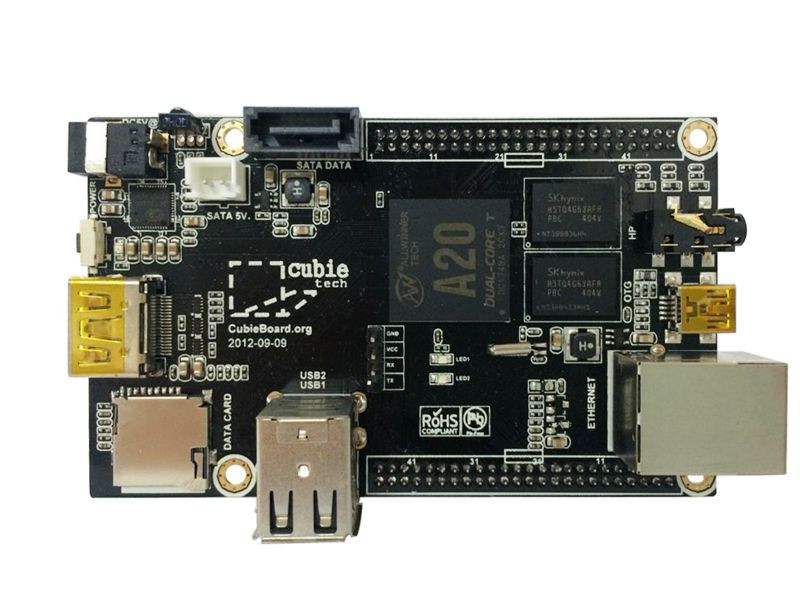
\includegraphics[width=2.5in]{cubieboard2}
\caption{Cubieboard 2}
\label{fig:plat_cb2}
\end{figure}

\begin{figure}[!t]
\centering
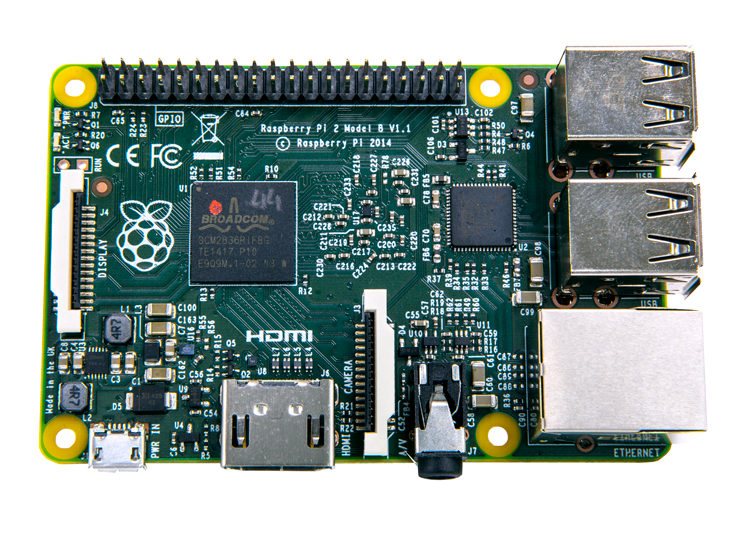
\includegraphics[width=2.5in]{RaspberryPi2}
\caption{Raspberry PI 2}
\label{fig:plat_rpi2}
\end{figure}

\section{Segmentação de Imagem}

Na figura \ref{fig:algoritmo} é ilustrado o diagrama em blocos do algoritmo de segmentação de objetos implementado nesse artigo baseado no trabalho  proposto por Horpraset \textit{et al.} \cite{IEEEhowto:horprasert}. Neste algoritmo é feita uma modelagem que   separa a imagem em duas componentes principais: brilho e cromaticidade. a primeira etapa do processo de segmentação é a modelagem do fundo, classificando cada pixel quanto à cor esperada, seu desvio padrão de cor e variações de distorção de brilho (\(\alpha\)) e distorção de cor (CD). Na sequência é feita a normalização dos histogramas de e CD, uma vez que essas grandezas não apresentam distribuições gaussianas. A partir dessas distribuições são estabelecidos os limiares de comparação que são utilizados na etapa de classificação de cada elemento de imagem. Dessa maneira  é possível fazer a classificação dos pixels com pertencentes as seguintes categorias: imagem de Fundo Original (B), Sombra (S), e Objeto  (F), das quais a última é a de principal interesse, mapeando a localização da imagem que apresenta os limiares desejados de CD para a extração do satisfatória da imagem de fundo. Toda etapa de modelagem da imagem de fundo é realizado sem a presença de objetos em movimento. São capturados 16 quadros para obtenção dos parâmetros desse modelo. Durante a etapa de classificação, para cada pixel da imagem corrente é efetuado o cálculo da distorção de cor e brilho que são comparados com os limiares previamente estabelecidos na etapa de aprendizado a fim de destacar os elementos de imagem pertencentes ao objeto.


O algoritmo supracitado foi implementado na linguagem Python, que tem sido largamente utilizada em computação científica devido a características como sintaxe simplificada, modularidade, tipagem dinâmica, gerênciamento de memória automático dentre diversos outros recursos \cite{IEEEhowto:fangohr}. Utilizou-se também como arcabouço básico as bibliotecas Numpy, que disponibiliza recursos de algebra linear, e a biblioteca OpenCV que dispõe de recursos para manipulação de imagens. A seguir podem ser observadas as primeiras linhas do \textit{script} desenvolvido, onde é possível ver a importação das referidas bibliotecas bem como a definição e configuração da resolução do dispositivo de captura de imagem:

\lstinputlisting[firstline=2, lastline=9]{horprasert_rgb_image_cam.py}

\begin{figure}[!t]
\centering
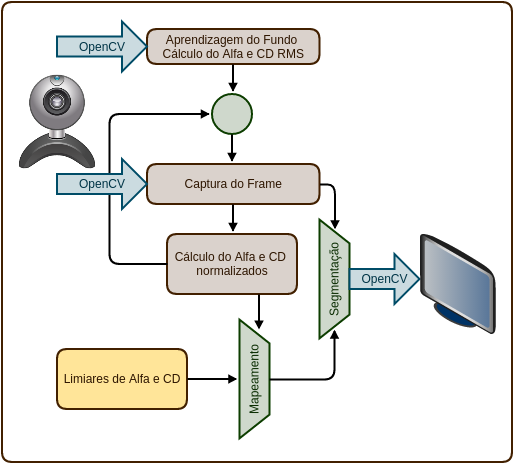
\includegraphics[width=2.5in]{Algoritmo}
\caption{Algoritmo de Segmentação de Imagem}
\label{fig:algoritmo}
\end{figure}

Em linux, o driver responsável por comunicar com dispositivos de vídeos é o \textit{Video For Linux - V4L2}, através do qual é possível acessar uma série de configurações da câmera utilizada com o auxílio da aplicação \textit{v4l2-ctl}. Essas configurações permitem a fixação de alguns parâmetros, que normalmente são alterados dinamicamente em câmeras comuns, e que, portanto, prejudicam a análise de segmentação da imagem, uma vez que isso é feito com base em uma imagem prévia de fundo e seus respectivos histogramas de desbalanço de cor e cromaticidade. Desse modo, fixando parâmetros críticos, como Exposição e Saturação, foi possível obter uma boa estabilidade no processo de detecção de objetos e remoção do fundo, abaixo são mostrados os comandos responsáveis por fixar os referidos parâmetros:

\lstinputlisting[firstline=2, lastline=9]{config_cam.py}

\section{Resultados}
As figuras \ref{fig:sim_pc} e \ref{fig:sim_rpi} mostram o resultado da execução do programa na CubieBoard 2 e em um Raspberry Pi 2, respectivamente. Na CB2 foi utilizado como câmera a webcam usb KLIP KDC-600 com resolução de 2M pixels enquanto que no RPI2 foi utilizado um módulo de câmera próprio com resolução de 5M pixels para a plataforma com como fonte de imagens. A Tabela \ref{tab:table_cb2} mostra os parâmetros estatísticos obtidos a partir de uma simulação com o processamento de 728 frames executada na CB2, enquanto que  a tabela \ref{tab:table_rpi} mostra os mesmos parâmetros para uma simulação utilizando o RPI2 com 728 amostras.

\begin{figure}[!t]
\centering
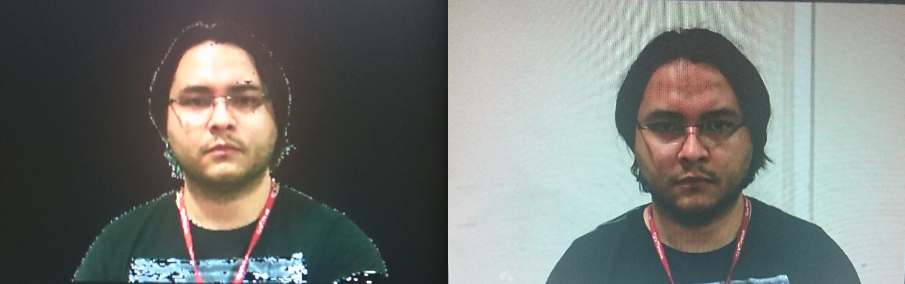
\includegraphics[width=2.5in]{resultado_cb2}
\caption{Resultado na simulação na Cubieboard 2}
\label{fig:sim_pc}
\end{figure}

\begin{figure}[!t]
\centering
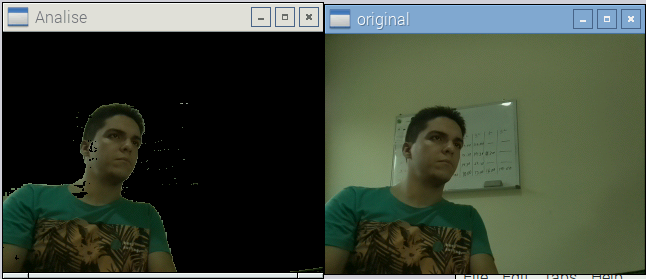
\includegraphics[width=2.5in]{Screen_RPI_01}
\caption{Resultado de simulação no Raspberry PI 2}
\label{fig:sim_rpi}
\end{figure}

Com base nos resultados obtidos fica evidente o impacto das restrições de processamento da CB2 e RPI2 nas métricas da aplicação, no entanto, a diferença entre as duas plataformas é pequena como mostram as tabelas \ref{tab:table_cb2} e \ref{tab:table_rpi}, onde observa-se que a média de quadros por segundo (fps - \textit{frames per second}) é pouco menor no RPI2. As figuras \ref{fig:processamento_cb2} e \ref{fig:processamento_rpi} mostram a divisão do processamento com base nas médias de tempo necessário para a captura, processamento e visualização da imagem. Observa-se que na CB2, com um pouco mais recursos de processamento, o cálculo e segmentação do frame responde por pouco mais de 96\% enquanto que no RaspberryPi supera a marca de 98\% do tempo de processamento.


\begin{table}[h]\centering
\renewcommand{\arraystretch}{1.75}
\caption{Resultados de Testes CB2 - 728 Amostras}
\label{tab:table_cb2}
\begin{tabular}{|c|c|c|c|c|}
\hline
\textbf{Parâmetro} & \textbf{fps} & \textbf{Captura (ms)} & \textbf{Calc (ms)} & \textbf{Show (ms)} \\\hline \hline
Média			& 5.656	& 5.445		&	170.71	&	1.47	\\ \hline
Desv. Padrão	& 0.417	& 1.306		&	12.277	&	0.169	\\ \hline
Máximo			& 6.873	& 12.475	&	196.18	&	2.100	\\ \hline
Mínimo			& 4.928	& 4.463		&	139.550	&	1.223	\\ \hline
\end{tabular}
\end{table}

\begin{table}[h]\centering
\renewcommand{\arraystretch}{1.75}
\caption{Taxa de Quadros por segundo no CB2 com multiprocessamento}
\label{tab:table_cb2_cores_fps}
\begin{tabular}{|c|c|c|c|c|}

\hline
\textbf{Núcleos} & \textbf{Média} & \textbf{Desvio Padrão} & \textbf{Máximo} & \textbf{Mínimo} \\\hline \hline
1		& 6.254		& 0.985		&	7.887	&	4.652	\\ \hline
2		& 15.25		& 20.58		&	118.27	&	3.057	\\ \hline

\end{tabular}
\end{table}

\begin{table}[h]\centering
\renewcommand{\arraystretch}{1.75}
\caption{Resultados de Testes no RPI2 - 728 Amostras}
\label{tab:table_rpi}
\begin{tabular}{|c|c|c|c|c|}

\hline
\textbf{Parâmetro} & \textbf{fps} & \textbf{Captura (ms)} & \textbf{Calc (ms)} & \textbf{Show (ms)} \\\hline \hline
Média			& 5.733 & 1.594	&	176.295	&	1.254	\\ \hline
Desv. Padrão	& 0.903 & 0.304	&	31.113	&	0.038	\\ \hline
Máximo			& 7.555 & 2.457 &	344.158	&	1.584	\\ \hline
Mínimo			& 2.878 & 1.057 &	129.112	&	1.207	\\ \hline

\end{tabular}
\end{table}

\begin{table}[h]\centering
\renewcommand{\arraystretch}{1.75}
\caption{Taxa de Quadros por segundo no RPI2 com multiprocessamento}
\label{tab:table_rpi_cores_fps}
\begin{tabular}{|c|c|c|c|c|}

\hline
\textbf{Núcleos} & \textbf{Média} & \textbf{Desvio Padrão} & \textbf{Máximo} & \textbf{Mínimo} \\\hline \hline
1		& 4.647		& 0.637		&	5.840	&	1.283	\\ \hline
2		& 9.999		& 6.262		&	60.557	&	4.458	\\ \hline
3		& 17.747	& 19.065 	&	96.119	&	3.972	\\ \hline
4		& 22.541	& 22.972	&	94.557	&	3.567	\\ \hline

\end{tabular}
\end{table}


\begin{figure}[!t]
\centering
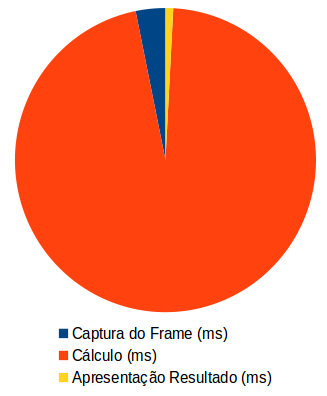
\includegraphics[width=2.0in]{Grafico_processamento_cb2_single_core}
\caption{Divisão de Processamento CB2 (Single Core)}
\label{fig:processamento_cb2}
\end{figure}

\begin{figure}[!t]
\centering
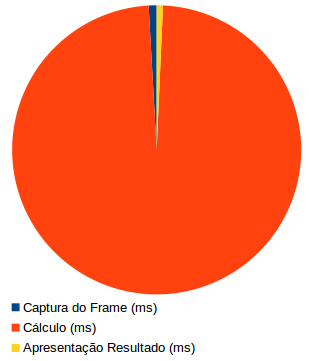
\includegraphics[width=2.0in]{Grafico_processamento_rpi2_single_core}
\caption{Divisão de Processamento RPI2 (Single Core)}
\label{fig:processamento_rpi}
\end{figure}


\newpage
Uma das razões para a característica observada é o fato de que o Python foi desenvolvido para ser executado em apenas um núcleo do processador, simplificando diversas questões inerentes à sistemas multiprocessados. No entanto, observando as restrições apresentadas pela aplicação no RPI2, foi feita a alteração no algoritmo para que o processamento fosse feito em mais de um núcleo, visando aumentar a taxa de quadros por segundo. A estratégia empregada se baseou na utilização do módulo \textit{Multiprocessing} do Python, que conforme descrito em \cite{IEEEhowto:micha} permite que processos da mesma aplicação sejam executados em núcleos distintos. A dificuldade fica por conta da necessidade de esses processos trocarem informação entre si, uma vez que são contextos completamente separados. A solução adotada foi a utilização de \textit{Queues} para enfileirar frames obtidos da câmera para serem processados e o mesmo tipo de estrutura para enfileirar o frame resultante de cada processo de segmentação para posterior exibição ao usuário. 

As tabelas \ref{tab:table_cb2_cores_fps} e \ref{tab:table_rpi_cores_fps} mostram o resultado da taxa de quadros por segundo para diferentes quantidades de núcleos de processamento CB2 e RPI2 respectivamente. Observa-se que com a utilização de mais de um núcleo foi possível melhorar significativamente a taxa de quadros por segundo.

Observando-se os resultados visuais obtidos em função das correções automáticas da câmera e do próprio ruído gerado durante a captura das imagens houve alguns falsos positivos, isto é, elementos de imagem que pertencem a imagem de fundo que foram classificados como objetos e dinamicamente são modificados em função do objeto no cenário. Estes falsos positivos foram observados com maior frequência na CB2 por se tratar de uma webcam convencional com ajuste automático de foco. No entanto, a segmentação mostrou-se robusta no cenário de testes utilizado e não apresentou rastros de movimento, pois a taxa de processamento foi acima de 15 quadros por segundo.



\section{Conclusão}
Foi possível observar a grande quantidade de recursos disponibilizada pela linguagem Python, com destaque para as ferramentas de manipulação de imagens e de matrizes, que são de grande importância para o estudo em visão computacional. Outro ponto bastante interessante foi a portabilidade das aplicações desenvolvidas com base nessa linguagem, de modo que nenhuma alteração se fez necessária quando da execução do \textit{script} desenvolvido nas duas plataformas embarcadas.

No entanto, ficaram bastante claras as limitações da plataforma CB2 e RPI2 devido à drástica queda na taxa de quadros processados por segundo quando utilizando apenas um núcleo. Considerando tal fator, foi avaliada a utilização de processamento paralelo, fazendo uso de todos os núcleos de processamento disponíveis na plataforma embarcada. Foi então observado que o aumento da média de quadros por segundo acompanhou linearmente o número de núcleos utilizados mesmo a despeito dos \textit{overheads} inerentes às estruturas de trocas de dados entre processos.

Observa-se, portanto, que é viável a utilização de uma plataforma com processador ARM para a execução de uma aplicação de processamento de vídeo em tempo real, sendo bastante razoável para aplicações com exigências mínimas de 15 quadros por segundo, uma vez que foi possível a obtenção de taxas superiores a 20 fps. 


\begin{thebibliography}{1}

\bibitem{IEEEhowto:sobral}
A.~Sobral, \emph{BGSLibrary: An OpenCV C++ Background Subraction Library}, \hskip 1em plus
  0.5em minus 0.4em\relax Salvador, Brasil: UFBA, 2013.

\bibitem{IEEEhowto:parolin}
A.~Parolin, \emph{Segmentação de Imagens de Pessoas em Tempo Real para Videoconferências}, \hskip 1em plus
  0.5em minus 0.4em\relax São Leopoldo, Brasil: UNISINOS, 2011.

\bibitem{IEEEhowto:oliveira}
J.P.~Oliveira, \emph{FPGA Architecture for Object Segmentation in Realtime}, \hskip 1em plus
  0.5em minus 0.4em\relax Florence, Italy: EUSIPCO, 2006.
  
\bibitem{IEEEhowto:horprasert}
T.~Horprasert et al., \emph{A Statistical Approach for Real-time Robust Background Subtraction and Shadow Detection}, \hskip 1em plus
  0.5em minus 0.4em\relax College Park, USA: University of MarylFand, 1999.
  
\bibitem{IEEEhowto:fangohr}
H.~Fangohr, \emph{Introduction to Python for Computational Science and Engineering}, \hskip 1em plus
  0.5em minus 0.4em\relax Southampton, England: University of Southampton, 2015.
  
\bibitem{IEEEhowto:micha}
H.~Fangohr, \emph{High Performance Python - Practical Performant Programming for Humans}, \hskip 1em plus
  0.5em minus 0.4em\relax Gravestein Highway North, California, USA: O'Reilly Media, 2014.

\end{thebibliography}



% that's all folks
\end{document}


